This Section explains the method and principles used for the system evaluation processes, measuring and comparing the performance (latency, in seconds, and throughput, in rows/second) of reading and writing Hudi and Iceberg tables on \gls{HopsFS}. Those operations are conducted respectively on the current legacy system and on the PyIceberg-based system, integrated in this thesis work.

\subsection{Evaluation process - RQ1 - Hudi vs. Iceberg}
\label{subsec:eval_process_hudi_iceberg}
This evaluation process will follow a sequential approach described in Figure~\ref{fig:method_experiments}. Each step of this process is related to one of the \glspl{G}~3-6 associated with the \gls{RQ}~1 in Section \ref{sec:intro_goals}, to which this process partially answer. The relationships between each process activity and \glspl{G} are here explained:
\begin{enumerate}
    \item \textbf{Design experiments}: this activity maps perfectly to \gls{G}~3, designing the experiments that will be conducted to evaluate the performance difference in performance between the current legacy access to Apache Hudi compared to the PyIceberg library-based access to Icbeerg Tables in \gls{HopsFS}. 
    \item \textbf{Perform experiments}: this activity maps perfectly to \gls{G}~4, using the integration detail (\gls{D}3-partial) to develop and conduct the designed experiments on the analyzed systems. Here, data is collected as latency, expressed in seconds.
    \item \textbf{Transform data according to metrics}: this activity is requisite to fulfill \gls{G}~5, and \gls{G}~8 of \gls{RQ}~2. The activity is conducted because throughput is not directly measured, but it is computed from latency following the formula here below:
    \[ Throughput \; (rows/second) = \frac{Number \; of \; rows \; (rows)}{Latency \;(seconds)}\]
    \item \textbf{Visualize results}: this activity maps perfectly to \gls{G}~5, visualizing the experiments' result according latency, measured in seconds, and throughput, measured in rows/second. This activity also generates \gls{D}~1, the experiment results complemented with tables and histograms, presented in Chapter \ref{ch:results_and_analysis}.
    \item \textbf{Analyze results}: this activity maps perfectly to \gls{G}~6, analyzing and interpreting the results delivered in \gls{D}~1. This activity contributes to \gls{D}~3, generating the analysis of experimental results, presented in Chapter \ref{ch:results_and_analysis}.
\end{enumerate}
\begin{figure}[!ht]
    \begin{center}
    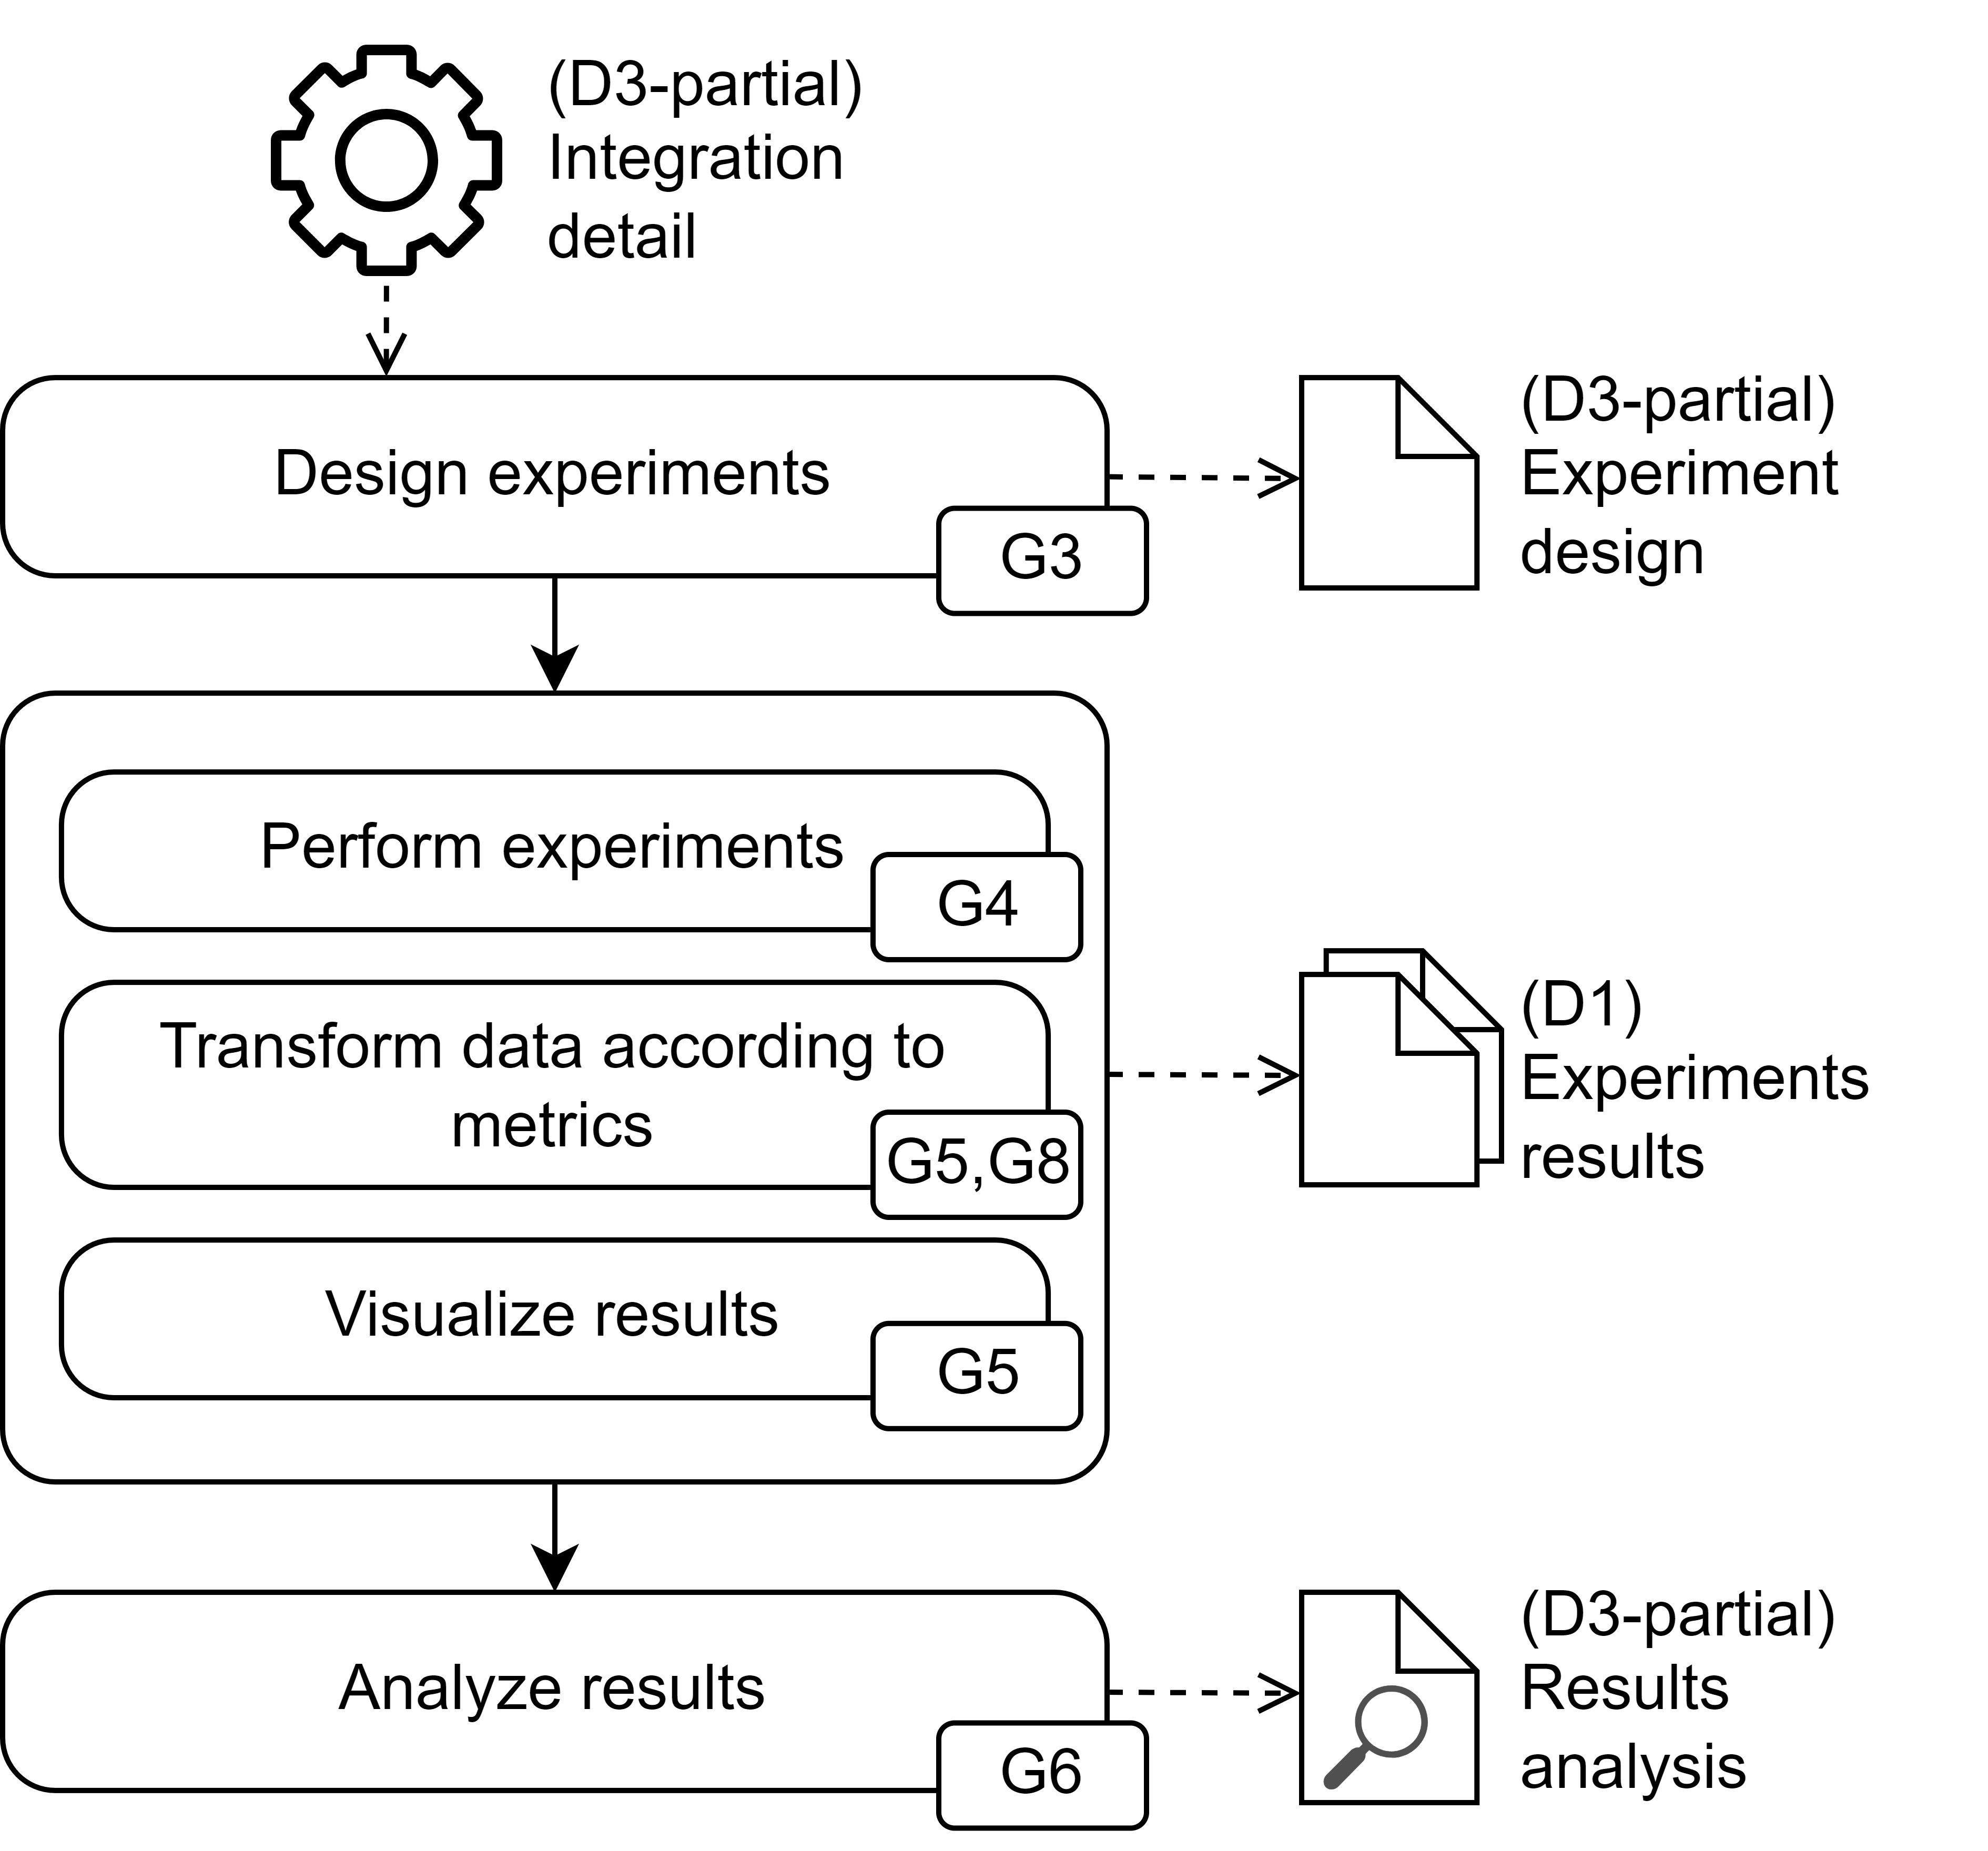
\includegraphics[width=0.8\textwidth]{figures/3-method/method_exp.png}
    \caption[System evaluation process - Hudi vs. Iceberg]{Diagram of the system evaluation process partially answering \gls{RQ}~1. Each activity is associated to specific \gls{G}. The process produces two \glspl{D}, the experiments results (\gls{D}~1) and a results analysis (\gls{D}3-partial).}
    \label{fig:method_experiments}
    \end{center}
\end{figure}


%%%% INDUSTRIAL USE CASE
\subsection{Industrial use case}
\label{subsec:method_use_case}

Several choices must be made for a system evaluation: which data will be used, which environment will run the experiments, and which metrics will be used to evaluate the system. Those choices depends on the scenarios for which the system is created. Thus, this Subsection describes the typical use case for this system. Follwing, the other Subsections describe which were the decision taken accordingly. While conducting their research in Hopsworks, the author outlined a typical industrial use case for the Hopsworks feature store, by reading internal documentation and discussing with several employees on their customer needs and trends. The use case is described by:
\begin{itemize}  
  \item \textbf{Table size}: most of the Hospworks' customers' workloads were limited (from 1M to 100M rows), with only few clients needing support for massive workloads (more than 1BN rows). Thus, this project opted to improve performance for the smaller workloads (from 100k to 100M rows). The datatset selected are presented in Section~\ref{subsec:experimental_data}.
  \item \textbf{Type of data}: the Hopsworks feature store works only with structured data (e.g., numbers, strings), thus experiment design and selected datasets embody this scenario.
  \item \textbf{Rows over storage size}: In the experimental part of this thesis, in order to have a realible unit measures for table size, the number of rows will be over the storage size (bytes). Perhaps, in the structured data domain of this use case, storage size (bytes) is neither linked to a table structure nor to a storage structure, arguably making this not reliable (i.e, table with a lot of rows and few columns, and a table with few ros and a lot of columns occupies the same memory).
  \item \textbf{Client configuration}: the client configuration is modeled to reflect typical customers' clients' computational and storage capabilities. Thus, the configuration are limited between one and eight \gls{CPU} cores, \gls{RAM} just sufficient for system needs and common \gls{SSD} storages. The experimental environment is further detailed in Section~\ref{subsec:experimental_env}.
\end{itemize}



%%%% EXPERIMENTAL DATA %%%%
\subsection{Experimental data}
\label{subsec:experimental_data}

The datasets that will be used to perform read and write experiments come from \glsentryshort{TPC}-H benchmark suite~\footnote{Benchmark suite website available at \url{https://www.tpc.org/tpch/}}. \glsentryshort{TPC}-H is a decision support benchmark by \gls{TPC}, that consists in a collection of business-oriented queries in specific industry sectors \cite{transactionprocessingperformancecounciltpcTPCH_v301pdf1993}, which became the de-facto standard for experiments on data storage system. Perhaps, it has been used in related studies \cite{raasveldtDuckDBEmbeddableAnalytical2019,behmPhotonFastQuery2022,manfrediReducingReadWrite2024}. 

The \glsentryshort{TPC}-H benchmark contains eight tables, and any part of the data can be generated via the \gls{TPC}-H data generation tool~\footnote{Available at \url{https://www.tpc.org/tpc_documents_current_versions/current_specifications5.asp}}. The two tables that will be used are the SUPPLIER and the LINEITEM, respectively, the smallest (10k rows) and largest (60M rows) tables. The size (number of rows) of a table depends on the \gls{SF}, that can be varied to progressivly change in the table size. The SUPPLIER table has seven columns, while the LINEITEM table has sixteen. This difference influences the average size of memory each row occupies. Below for each table their columns are listed, specifying which data type they store.
\begin{itemize}
  \item SUPPLIER
  \begin{itemize}
    \item S\_SUPPKEY : identifier
    \item S\_NAME : fixed text, size 25
    \item S\_ADDRESS : variable text, size 40
    \item S\_NATIONKEY : identifier
    \item S\_PHONE : fixed text, size 15
    \item S\_ACCTBAL : decimal
    \item S\_COMMENT : variable text, size 101
  \end{itemize}
  \item LINEITEM
  \begin{itemize}
    \item L\_ORDERKEY : identifier
    \item L\_PARTKEY : identifier
    \item L\_SUPPKEY : identifier
    \item L\_LINENUMBER : integer
    \item L\_QUANTITY : decimal
    \item L\_EXTENDEDPRICE : decimal
    \item L\_DISCOUNT : decimal
    \item L\_TAX : decimal
    \item L\_RETURNFLAG : fixed text, size 1
    \item L\_LINESTATUS : fixed text, size 1
    \item L\_SHIPDATE : date
    \item L\_COMMITDATE : date
    \item L\_RECEIPTDATE : date
    \item L\_SHIPINSTRUCT : fixed text, size 25
    \item L\_SHIPMODE : fixed text, size 10
    \item L\_COMMENT : variable text, size 44
  \end{itemize} 
\end{itemize}

Considering the different structure of the two tables used (i.e., number of columns and data types) comparison across different tables cannot be done using the the selected metrics, i.e., latency (seconds) and throughput(rows/second). For this reason, the system evaluation will only consider same tables on different configuration. This project used five table variations to benchmark the system integration. \gls{SF} was varied to obtain a table at each significant order of magnitude, from 10k rows to 60M rows. These are the tables:
\begin{enumerate}
    \item \textit{supplier\_sf1}: size = 10000 rows
    \item \textit{supplier\_sf10}: size = 100000 rows
    \item \textit{supplier\_sf100}: size = 1000000 rows
    \item \textit{lineitem\_sf1}: size = 60000000 rows
    \item \textit{lineitem\_sf10}: size = 60000000 rows
\end{enumerate}

Lastly, despite no information are given about the row and storage size (bytes) ratio, in accordance to Section \ref{subsec:method_use_case}, this Section presentes comprehensive information on the data, including how to retrieve it and how it is composed. These gives to the reader the ability of calculating the storage occupancy of each table, depending on their prefered unit of measure.



%%%% EXPERIMENTAL DESIGN
\subsection{Experimental design}
\label{subsec:experimental_design}



%%%% EXPERIMENTAL ENVIRONMENT
\subsection{Experimental environment}
\label{subsec:experimental_env}



%%%% EVALUATION FRAMEWORK
\subsection{Evaluation framework}
\label{subsec:method_eval_framework}


%%%% RELIABILITY AND VALIDITY
\subsection{Reliability and validity}
\label{subsec:method_reliability_validity}